\section{Objective, derivatives, and counting identities}\label{app:derivation}
Write $L(\theta;y,w)=\sum_r w_r[\log(1+\exp(x_r^\top\theta))-y_rx_r^\top\theta]+\lambda\|\theta\|^2/2$, with all original $w_r=1$ and $\lambda>0$. The gradient and Hessian are
\begin{align}\label{eq:grad}
 g(\theta)&=\sum_r w_rx_r(p_r-y_r)+\lambda\theta,\\
 H(\theta)&=\sum_r w_rp_r(1-p_r)x_rx_r^\top+\lambda I.\label{eq:hessian}
\end{align}
For nonnegative weights, $H$ is positive definite. The loss is smooth and coercive because of the positive quadratic penalty, so a unique finite minimizer exists. Summing the gradient coordinates gives $\lambda\sum_i\widehat\theta_i=0$. This justifies centered coordinates without an arbitrary reference entrant.

For a single record, continuously interpolate its outcome as $y_r(t)=y_r+t(1-2y_r)$, holding weights fixed. Differentiating $g(\widehat\theta(t),t)=0$ at $t=0$ gives
\begin{equation}\label{eq:flipderivative}
 H\frac{d\widehat\theta}{dt}+x_r(2y_r-1)=0,
 \qquad -\frac{dm}{dt}=c^\top H^{-1}x_r(2y_r-1).
\end{equation}
For deletion, use $w_r(t)=1-t$ and fixed response. The corresponding derivative is
\begin{equation}\label{eq:delderivative}
 H\frac{d\widehat\theta}{dt}-x_r(p_r-y_r)=0,
 \qquad -\frac{dm}{dt}=c^\top H^{-1}x_r(y_r-p_r).
\end{equation}
The actual discrete operation uses $t=1$, for which this derivative need not approximate the full refit accurately. Positive-score sorting optimizes only the additive first-order objective. The ridge term remains in the Hessian and is not removed or rescaled after deletion. These standard implicit derivatives are implementation identities, not a novel influence theorem.

For exposure, $\sum_i n_i=2N$ and $\sum_i k_i(S)=2|S|$, because each retained comparison has exactly two distinct endpoints. Substitution proves Eq.~\eqref{eq:exposure}; a weighted average cannot exceed the maximum of its terms. Summing strict capacities and dividing by two proves Eq.~\eqref{eq:countbound}; the integer floor follows because $|S|$ is integral. This count bound does not depend on any fitted score or attack heuristic. It is generally not tight when endpoint pairs, beneficial outcomes, or other constraints limit feasibility.

\paragraph{Numerical implementation.}
We aggregate counts and response sums for each canonical unordered pair; this is exact for Eq.~\eqref{eq:bt}, including fractional responses. Newton steps solve the dense positive-definite system using SciPy, with backtracking and a default maximum gradient target $10^{-8}$. A fit fails if its final gradient exceeds $2\times10^{-6}$ or has a nonfinite state; no such production failure occurred. Canonical orientation is checked at the data boundary because lower-triangle inputs would otherwise be silently omitted by upper-triangle sufficient statistics. Analytical two-player and finite-difference gradient, Hessian, outcome, and deletion tests are supplied, along with integer-surrogate brute force on a toy example. The toy fixture is a unit test, not experimental synthetic evidence.

For the integer-linear control, one bounded integer variable counts selected records in an observed $(a,b,y)$ class; all members have equal influence. Endpoint incidence constraints and a global cardinality constraint are linear. SciPy's mixed-integer solver uses a 60-second limit and relative gap target $10^{-9}$; every recorded condition terminates with status zero and reported gap zero. Refitted margins remain feasible nonlinear witnesses only. Different equal-objective class allocations can produce different discrete sets or counts.

\section{Data snapshots, provenance, and edit semantics}\label{app:data}
The data owners are LMArena/LMSYS for Arena, the MT-Bench authors for the judgment release, and FiveThirtyEight for the NBA archive. We downloaded only the fixed public snapshots specified in the task. Table~\ref{tab:sources} records the commits and terms; the code's \texttt{artifacts/data\_manifest.json} records exact resolve URLs, bytes, and SHA256 values for all four source files. Three supplied hashes are checked before parsing; the fourth (GPT-4 parquet) is computed and recorded. Raw data remain in \texttt{data/} and are excluded from the reproduction archive.

\begin{table}[h]
\centering\small
\caption{Source snapshots. Dataset cards and repository license were fetched directly and retained in the provenance bundle. No third-party rehosting or restricted dataset is needed.}\label{tab:sources}
\begin{tabular}{p{.17\linewidth}p{.57\linewidth}p{.17\linewidth}}
\toprule
Source & Public repository and fixed commit & License\\
\midrule
Arena55k & \url{https://huggingface.co/datasets/lmarena-ai/arena-human-preference-55k}; \texttt{18c298340948c0e7f7727399fd459cca6ce0ca6f} & Apache-2.0\\
MT human / GPT-4 & \url{https://huggingface.co/datasets/lmsys/mt_bench_human_judgments}; \texttt{f7d2896d2cc5d80f8b55c2bbc722613555233c25} & CC-BY-4.0\\
NBA historical & \url{https://github.com/fivethirtyeight/data}; \texttt{4c1ff5e3aef1816ae04af63218015066e186c147}; \texttt{nba-elo/nbaallelo.csv} & CC-BY-4.0\\
\bottomrule
\end{tabular}

\end{table}

Arena uses all eligible rows and all observed models, with no outcome-based top-model trimming. Winner columns are checked to sum to one; self comparisons and invalid winners would be excluded and counted. The retained full snapshot has no such exclusions or duplicate record IDs. Prompt content is used only for exact-string hashing to define resampling clusters; no conversations are quoted or redistributed. The term ``55k'' is the public dataset label rather than the exact retained count in Table~\ref{tab:data}.

MT processing maps observed winner labels to $1,0,0.5$ and canonicalizes model orientation before aggregation. There are 380 GPT-4 records labeled \texttt{tie (inconsistent)}, distinct from 220 explicit ties; the main fit includes both as half outcomes. The human source restrictions select the observed \texttt{expert\_} versus \texttt{author\_} label prefix without inferring identities. \texttt{mt\_human\_cell\_provenance.csv} and its GPT-4 counterpart retain question, turn, unordered pair, multiplicity, number of distinct judges, and source row indices, sufficient to reconstruct each aggregate without redistributing conversations. Each common cell is weighted equally, regardless of its human judgment multiplicity. Matched-cell response reversals invert the entire mean; their nominal cell budgets are not raw-vote budgets.

For NBA, filter league NBA and the three fixed \texttt{year\_id} values, then retain \texttt{\_iscopy==0}. Game IDs are verified unique. A game outcome is one binary comparison; the mirrored opponent row is not a second observation. Historical records are used as a cross-domain test of a static score aggregation, not to infer current team ability, home advantage, or misconduct.

\section{Uncertainty details and additional controls}\label{app:uncertainty}
Each original-data replicate samples the same number of clusters as observed, with replacement, and assigns every row its cluster multiplicity as a likelihood weight. The pair remains fixed to the full-data leader/runner. The base seed is 20261104; original and exploratory bootstraps use seed base $+100000+b$, and random controls use base $+r$ or base $+200000+r$. Random sets at different nominal budgets share a permutation within a seed and are therefore nested, not independent across the budget curve. This coupling is deliberate and is not used for multiplicity-unadjusted significance tests.

\begin{table}[h]
\centering\small
\caption{Uncertainty at nominal 1\% on full cohorts. $s_0$: original margin SD. Win retention: original leader remains first under cluster bootstrap. Flip: random-subset pair-reversal frequency with Wilson 95\% interval (100 draws). Last column: empirical 2.5--97.5\% random edited-margin range, not an interval for an estimated mean.}\label{tab:uncertainty}
\begin{tabular}{lrrrrr}
\toprule
Cohort & $s_0$ & Win retain\% & Flip\% & Wilson interval\% & Random margin range \\
\midrule
Arena & 0.055 & 52.0 & 35 & [26.4, 44.7] & [-0.018, 0.038] \\
MT human & 0.136 & 100.0 & 0 & [0.0, 3.7] & [0.325, 0.401] \\
MT GPT-4 & 0.153 & 100.0 & 0 & [0.0, 3.7] & [0.726, 0.826] \\
NBA 2013 & 0.324 & 64.7 & 1 & [0.2, 5.4] & [0.069, 0.364] \\
NBA 2014 & 0.318 & 78.3 & 0 & [0.0, 3.7] & [0.152, 0.426] \\
NBA 2015 & 0.314 & 96.7 & 0 & [0.0, 3.7] & [0.568, 0.825] \\
\bottomrule
\end{tabular}


\end{table}

The count-matched control samples exactly as many non-tie records as the corresponding capped greedy set, without enforcing its endpoint restriction. Table~\ref{tab:controls} reports both supplementary random controls. The cap-feasible control shuffles priorities and accepts records greedily if both endpoint slots remain. It is a heuristic feasible sampler, not a uniform distribution over feasible sets or an equal-count control. Reporting their actual mean counts and exposure avoids conflating those roles.

\begin{table}[h]
\centering\small
\caption{Supplementary random controls at nominal 1\%. $D$ uses the same original SD as the primary analysis. Cap-feasible draws can underfill; count-matched draws need not satisfy the caps.}\label{tab:controls}
\begin{tabular}{llrrrr}
\toprule
Cohort & Random control & Mean edits & Mean $100\rho$ & Mean $D$ & 95\% subset range \\
\midrule
Arena & Count-matched & 555.0 & 2.07 & -0.014 & [-0.430, 0.413] \\
Arena & Cap-feasible & 557.0 & 1.00 & -0.020 & [-0.464, 0.365] \\
MT human & Count-matched & 29.0 & 1.19 & 0.085 & [-0.145, 0.320] \\
MT human & Cap-feasible & 31.2 & 0.99 & 0.107 & [-0.129, 0.338] \\
MT GPT-4 & Count-matched & 24.0 & 1.41 & 0.276 & [-0.029, 0.594] \\
MT GPT-4 & Cap-feasible & 23.4 & 1.00 & 0.247 & [0.003, 0.417] \\
NBA 2013 & Count-matched & 1.0 & 1.19 & 0.002 & [-0.138, 0.161] \\
NBA 2013 & Cap-feasible & 1.0 & 0.99 & 0.037 & [-0.311, 0.309] \\
NBA 2014 & Count-matched & 2.0 & 1.31 & 0.008 & [-0.140, 0.158] \\
NBA 2014 & Cap-feasible & 2.0 & 0.99 & -0.008 & [-0.300, 0.298] \\
NBA 2015 & Count-matched & 1.0 & 1.19 & 0.007 & [-0.144, 0.188] \\
NBA 2015 & Cap-feasible & 1.0 & 0.98 & 0.072 & [-0.182, 0.175] \\
\bottomrule
\end{tabular}


\end{table}

\paragraph{Matched contrast.}
The common panels contain the same question IDs and cell order; matching is by question, turn, and unordered pair. Synchronized bootstrap question draws therefore support a paired difference of the \emph{same} GPT-4-versus-Claude margin. This difference does not establish evaluator accuracy: there is no external ground truth for which model should have the larger gap. Unmatched full releases are not substituted for this paired target.

\clearpage
\section{Cap feasibility and specification stress tests}\label{app:stress}
Table~\ref{tab:feasibility} separates endpoint-slot arithmetic from the selected procedure's behavior. Table~\ref{tab:stress} compares the tested selection and rounding variants.
\begin{table}[h]
\centering\small
\caption{Primary strict-cap arithmetic. Eligible rows are non-ties whose two endpoints have positive capacities, before considering their influence signs. Count upper bound is Eq.~\eqref{eq:countbound}; edges may reduce feasibility further. In NBA this upper bound already explains the one/two/one selected counts.}\label{tab:feasibility}
\begin{tabular}{lrrrrr}
\toprule
Cohort & Global budget & Zero-cap entrants & Eligible rows & Count upper bound & Greedy edits \\
\midrule
Arena & 574 & 0 & 39716 & 559 & 555 \\
MT human & 33 & 0 & 2575 & 32 & 29 \\
MT GPT-4 & 24 & 0 & 1800 & 24 & 24 \\
NBA 2013 & 13 & 27 & 21 & 1 & 1 \\
NBA 2014 & 13 & 26 & 33 & 2 & 2 \\
NBA 2015 & 13 & 28 & 8 & 1 & 1 \\
\bottomrule
\end{tabular}


\end{table}

\begin{table}[h]
\centering\small
\caption{Exact edited fixed-pair margins at nominal 1\%. Adaptive U uses at most ten batches; Integer C optimizes the additive influence surrogate under strict caps. Cap+1 replaces every endpoint limit by $\lfloor\alpha n_i\rfloor+1$ while keeping the original global budget. Its larger realized $\rho$ demonstrates a changed restriction, not equivalent rounding.}\label{tab:stress}
\begin{tabular}{lrrrrrr}
\toprule
Cohort & Static U & Adaptive U & Greedy C & Integer C & Cap+1 & $100\rho_{{+1}}$ \\
\midrule
Arena & -1.244 & -1.244 & -0.100 & -0.101 & -0.106 & 2.00 \\
MT human & 0.101 & 0.101 & 0.294 & 0.294 & 0.286 & 1.08 \\
MT GPT-4 & 0.482 & 0.482 & 0.700 & 0.700 & 0.686 & 1.12 \\
NBA 2013 & -0.707 & -0.789 & 0.128 & 0.128 & -0.022 & 2.00 \\
NBA 2014 & -0.500 & -0.576 & 0.200 & 0.200 & 0.088 & 1.98 \\
NBA 2015 & -0.309 & -0.342 & 0.689 & 0.689 & 0.560 & 1.96 \\
\bottomrule
\end{tabular}


\end{table}

\begin{table}[h]
\centering\small
\caption{Uncapped 1\% checks retain the original full-cohort pair. Each specification has its own $N$, unedited fit, degrees, and floor budget. A ``Base reversed'' flag means the unedited altered specification already reverses that pair. NBA tie dropping changes no rows; it is intentionally a null ablation.}\label{tab:specifications}
\begin{tabular}{llrrrr}
\toprule
Cohort & Specification & $N$ & Unedited margin & Edited margin & Base reversed \\
\midrule
Arena & Ridge 0.01 & 57477 & 0.004 & -1.245 & 0 \\
Arena & Ridge 1 & 57477 & 0.008 & -1.231 & 0 \\
Arena & Drop exact ties & 39716 & -0.033 & -6.184 & 1 \\
MT human & Ridge 0.01 & 3355 & 0.378 & 0.101 & 0 \\
MT human & Ridge 1 & 3355 & 0.376 & 0.101 & 0 \\
MT human & Drop exact ties & 2575 & 0.532 & 0.208 & 0 \\
MT GPT-4 & Ridge 0.01 & 2400 & 0.821 & 0.482 & 0 \\
MT GPT-4 & Ridge 1 & 2400 & 0.809 & 0.476 & 0 \\
MT GPT-4 & Drop exact ties & 1800 & 1.100 & 0.563 & 0 \\
NBA 2013 & Ridge 0.01 & 1314 & 0.229 & -0.713 & 0 \\
NBA 2013 & Ridge 1 & 1314 & 0.219 & -0.652 & 0 \\
NBA 2013 & Drop exact ties & 1314 & 0.228 & -0.707 & 0 \\
NBA 2014 & Ridge 0.01 & 1319 & 0.297 & -0.504 & 0 \\
NBA 2014 & Ridge 1 & 1319 & 0.279 & -0.467 & 0 \\
NBA 2014 & Drop exact ties & 1319 & 0.295 & -0.500 & 0 \\
NBA 2015 & Ridge 0.01 & 1311 & 0.750 & -0.312 & 0 \\
NBA 2015 & Ridge 1 & 1311 & 0.693 & -0.285 & 0 \\
NBA 2015 & Drop exact ties & 1311 & 0.744 & -0.309 & 0 \\
\bottomrule
\end{tabular}


\end{table}

\begin{table}[t]
\centering\small
\caption{Observed judge-source and inconsistency-label sensitivities. U/C denote uncapped/strict capped outcome reversals. Different restrictions change the target record population, not merely an attack algorithm. They are exploratory descriptive checks.}\label{tab:semantics}
\begin{tabular}{llrrrrrr}
\toprule
Cohort & Restriction & $N$ & $m_0$ & U1\% & C1\% & U5\% & C5\% \\
\midrule
MT human & experts only & 2668 & 0.403 & 0.144 & 0.319 & -0.640 & -0.026 \\
MT human & authors only & 687 & 0.255 & -0.069 & 0.198 & -0.838 & -0.163 \\
MT GPT-4 & exclude inconsistent & 2020 & 0.992 & 0.548 & 0.833 & -0.774 & 0.264 \\
\bottomrule
\end{tabular}


\end{table}

Whole-question edits reverse every non-tie judgment in a selected MT question, across all observed pairs and turns. Question influence is the sum of row scores, and questions with beneficial total influence are selected in descending order. The question budget is separate from the changed-judgment budget; ties are touched but unchanged. These group edits are not constrained by the row-level endpoint caps. All costs and final margins are reported rather than equating a question with one vote.

\begin{table}[h]
\centering\small
\caption{MT whole-question reversals. Fractions use all 80 questions or the original full-release row count, respectively. ``Changed judgments'' excludes exact ties; touched-row counts are also retained in the source CSV.}\label{tab:groups}
\begin{tabular}{lrrrrr}
\toprule
Cohort & Questions & Question\% & Changed judgments & Row\% & Margin \\
\midrule
MT human & 1 & 1.25 & 39 & 1.16 & 0.274 \\
MT human & 2 & 2.50 & 88 & 2.62 & 0.173 \\
MT human & 4 & 5.00 & 173 & 5.16 & 0.036 \\
MT human & 8 & 10.00 & 320 & 9.54 & -0.209 \\
MT GPT-4 & 1 & 1.25 & 12 & 0.50 & 0.714 \\
MT GPT-4 & 2 & 2.50 & 26 & 1.08 & 0.615 \\
MT GPT-4 & 4 & 5.00 & 60 & 2.50 & 0.439 \\
MT GPT-4 & 8 & 10.00 & 120 & 5.00 & 0.147 \\
\bottomrule
\end{tabular}


\end{table}

\clearpage
\section{Approximation accuracy and observed grid witnesses}\label{app:approx}
Figure~\ref{fig:approx} audits finite-budget approximation errors; Table~\ref{tab:grid} lists the first observed grid witnesses without claiming minimum budgets.
\begin{figure}[h]
\centering
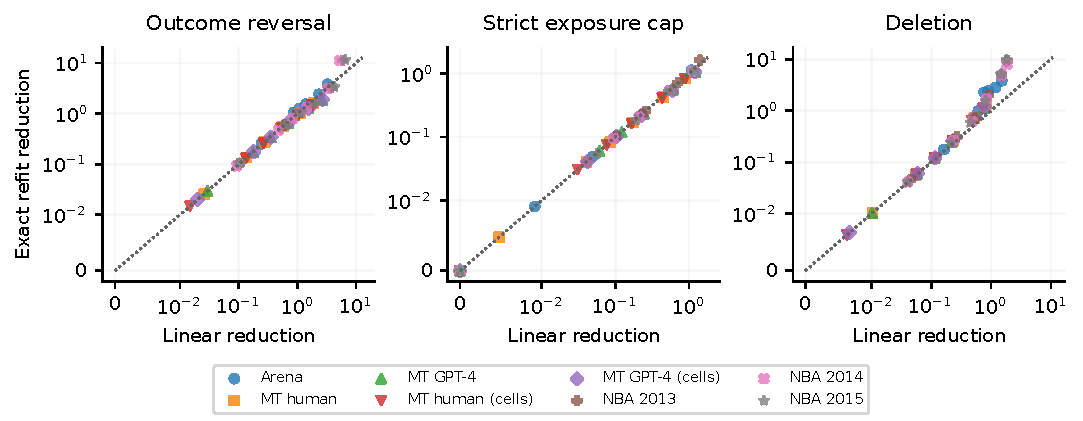
\includegraphics[width=\linewidth]{figures/approximation.pdf}
\caption{Exact-refit versus first-order predicted reductions for every nonzero grid budget and all eight cohorts. Both axes are symlog, linear within 0.01. The dotted line is equality, not a regression. Large finite-budget discrepancies, especially for deletions, preclude using a linearized ranking change as a certificate.}\label{fig:approx}
\end{figure}

\begin{table}[h]
\centering\small
\caption{First \emph{observed} pair reversal on the fixed nominal grid, not the minimum necessary budget. No intermediate budgets or alternative nonlinear edit sets are searched. Matched rows are aggregate-cell units, unlike full-release judgment/game units.}\label{tab:grid}
\begin{tabular}{lrrr}
\toprule
Cohort & Uncapped flip & Capped flip & Deletion \\
\midrule
Arena & 0.1\% & 0.1\% & 0.1\% \\
MT human & 2\% & 5\% & 5\% \\
MT GPT-4 & 5\% & 10\% & 10\% \\
MT human (cells) & 2\% & 5\% & 5\% \\
MT GPT-4 (cells) & 5\% & 10\% & 10\% \\
NBA 2013 & 0.5\% & 2\% & 0.5\% \\
NBA 2014 & 0.5\% & 5\% & 1\% \\
NBA 2015 & 1\% & 10\% & 2\% \\
\bottomrule
\end{tabular}


\end{table}

All deterministic primary and supplementary edit sets have compressed NPZ witnesses containing Unicode row IDs, canonical endpoints, original responses, and selected indices. They are loaded with \texttt{allow\_pickle=False}. The validator reconstructs the appropriate tie/source-restricted data specification and refits from a cold start. It also checks unique indices, exact original responses, nominal global counts, and strict endpoint limits. The current audit replays \R{auditreplayed} deterministic witnesses; the maximum recorded margin discrepancy is below $10^{-7}$. Numerical fit counts and gradients are separately reconciled for the primary, supplemental, and exploratory-bootstrap runs in \texttt{validation.json}. Random sets and bootstrap weights are regenerated from saved seeds and immutable data ordering rather than stored as fabricated witnesses.

\section{Exploratory end-to-end bootstrap}\label{app:boot}
This analysis was added after inspecting the production endpoints, and is explicitly separated from the locked primary plan. For each of 300 cluster draws, expand rows according to cluster multiplicity, refit the unedited data, recompute $N$, entrant degrees, the floor budget, influence ordering, and strict capacities, then select and refit new sets at 1\%. The original full-data contrast is retained, even if already reversed in the unedited resample. All fits use the same ridge as the primary analysis. The intervals describe the entire data-resampling/selection/refitting procedure, not one fixed selected set. No extra replicates were added to shift a percentile endpoint.

\begin{figure}[h]
\centering
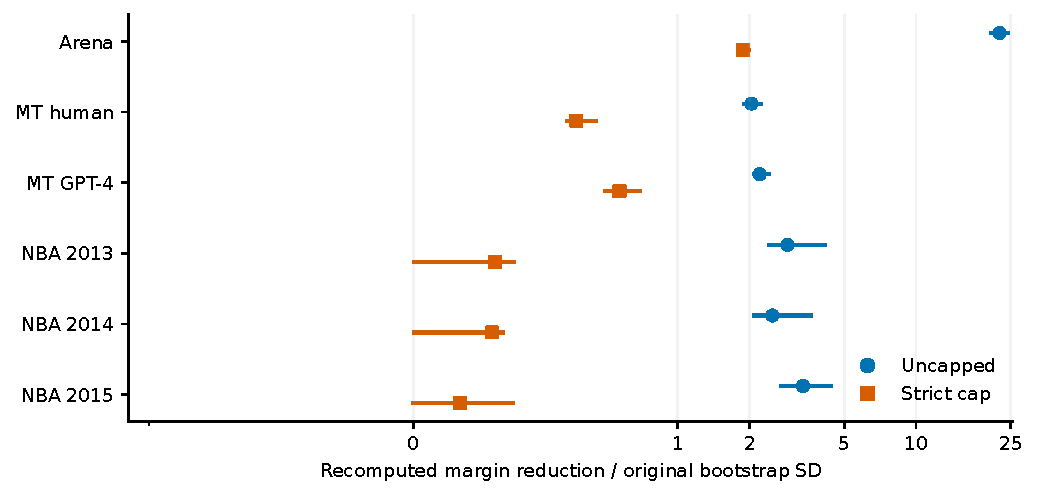
\includegraphics[width=\linewidth]{figures/bootstrap_effects.pdf}
\caption{Exploratory end-to-end effect distributions. Points are original-data reductions; whiskers are percentile reduction ranges from recomputed procedures, divided by the original fixed SD. Symlog horizontal scale is linear within one unit. These are not selection-adjusted intervals or post-edit significance tests.}\label{fig:boot}
\end{figure}

\begin{table}[h]
\centering\small
\caption{Raw-margin percentile intervals for the exploratory recomputed procedure. Reversed\% is the fraction of edited replicate margins below zero, not a frequentist guarantee or a conditional causal effect of editing. It can include resamples with an already reversed original pair.}\label{tab:boot}
\begin{tabular}{llrrr}
\toprule
Cohort & Selector & Reduction interval & Edited-margin interval & Reversed\% \\
\midrule
Arena & U & [1.152, 1.350] & [-1.353, -1.140] & 100.0 \\
Arena & C & [0.101, 0.110] & [-0.209, 0.001] & 97.0 \\
MT human & U & [0.259, 0.305] & [-0.176, 0.382] & 22.7 \\
MT human & C & [0.079, 0.094] & [0.021, 0.574] & 1.0 \\
MT GPT-4 & U & [0.319, 0.370] & [0.215, 0.754] & 0.0 \\
MT GPT-4 & C & [0.111, 0.131] & [0.430, 0.991] & 0.0 \\
NBA 2013 & U & [0.785, 1.339] & [-1.528, -0.190] & 99.3 \\
NBA 2013 & C & [0.001, 0.123] & [-0.486, 0.772] & 33.7 \\
NBA 2014 & U & [0.667, 1.154] & [-1.396, 0.106] & 95.0 \\
NBA 2014 & C & [0.001, 0.108] & [-0.427, 0.853] & 19.3 \\
NBA 2015 & U & [0.855, 1.385] & [-1.070, 0.215] & 87.3 \\
NBA 2015 & C & [0.000, 0.119] & [0.109, 1.326] & 1.0 \\
\bottomrule
\end{tabular}


\end{table}

\clearpage
\section{Reproducibility, compute, and failures}\label{app:reproduce}
The code archive contains \texttt{src/}, \texttt{tests/}, the pinned \texttt{requirements.txt}, \texttt{reproduce.py}, and a README with the data commands and script-to-table/figure map. Run \texttt{python reproduce.py} from the workspace root after installing the requirements; cached original data are checksum-verified. Individual commands are:
\begin{verbatim}
python src/download_data.py
python -m pytest tests -q
python src/run_experiments.py --bootstrap 300 --random 100
python src/run_stress.py --replicates 100
python src/bootstrap_sensitivity.py
python src/validate_results.py
python src/summarize.py
python src/plot_figures.py
python src/complete_checklist.py
latexmk -pdf -cd paper/main.tex
\end{verbatim}
Set \texttt{OPENBLAS\_NUM\_THREADS=1}, \texttt{OMP\_NUM\_THREADS=1}, and \texttt{MKL\_NUM\_THREADS=1} before execution. The numerical environment is Python 3.11.15, NumPy 2.4.6, SciPy 1.17.1, pandas 3.0.6, Matplotlib 3.11.2, PyArrow 26.0.1, pytest 9.2.0, and pypdf 6.21.4. PDF compilation used pdfTeX 1.40.26 (TeX Live 2025/dev/Debian) and the unmodified official NeurIPS 2026 style. The runtime exposes 40 logical CPUs but each numerical process requests one thread; the CPU model and host memory are not exposed through the permitted inspection interface. This does not imply the experiments used 40 cores.

\IfFileExists{resources.tex}{The final replay measured 17.3 seconds for the core experiment process, 17.2 seconds for supplemental controls, and 28.9 seconds for the exploratory bootstrap. The complete download-verification, test, analysis, validation, and rendering sequence took 80.4 seconds before PDF compilation. Peak child resident memory across these stages was 349.5 MiB (Linux cumulative child-process maximum RSS). These are measured times on the provided shared host, not guarantees for another machine. Original pilot and dependency-recovery costs are additional and are logged separately.
}{The machine-readable runtime metadata accompany the code; compilation of this provisional source predates the timed final replay.}

Every scientific CSV can be regenerated without a GPU or paid API. \texttt{summarize.py} produces all numerical tables and the claim ledger; \texttt{plot\_figures.py} reads those CSVs to produce every figure. \texttt{results\_macros.tex} is generated, not a source of invented result numbers. Sufficient-statistic fitting avoids storing a dense $N\times P$ design matrix. Download and TeX/dependency installation time are additional and network-dependent; the budget is comfortably below one CPU week for these snapshots, not a complexity guarantee for larger systems.

\paragraph{Failures and abandoned branches.}
The first NPZ replay failed because object-typed string IDs required unsafe pickle loading; IDs were changed to Unicode and all witnesses regenerated. No unsafe deserialization workaround was used. Initial PDF-extraction dependency recovery and a legacy template URL failure are logged separately; the official 2026 bundle was then obtained from the conference CFP. A blocked system-path CPU-model probe was not bypassed. Optional Arena matched-exposure subsampling was deferred. We did not train manipulation classifiers, call live judges, reproduce a published minimum-edit number, or run a causal evaluator-design experiment. Unsuccessful or unperformed branches are not represented as positive evidence.

\section{LLM assistance, licensing, and access boundaries}\label{app:llm}
An LLM-based research assistant, operating as EvoScientist, autonomously selected the study design, consulted the allowed literature, wrote and tested analysis code, interpreted measured results, and drafted the manuscript. Subagents supplied literature notes, stage critique, and manuscript self-review. The runtime did not expose a verified underlying model identifier; none is invented here. LLM reasoning is not an empirical measurement or mathematical certification: all reported data values, tables, and plotted points are computed by the included CPU programs. No paid inference API, newly generated judge labels, or GPU was used. A human scientific and legal review remains appropriate before actual submission.

New analysis code is supplied under the MIT license; third-party datasets, official style files, and consulted papers retain their original terms. Derived audit summaries and row-ID witnesses do not relicense underlying assets. Raw conversations, all original data files, and third-party paper PDFs are excluded from distribution archives; the source/provenance manifests identify how to obtain them legitimately. The official 2026 checklist is retained with all sixteen answers and justifications.

\subsection{Restricted-access protocol}\label{app:access}
The task specified an unidentified prior paper and prohibited access to it and to pages discussing it, while explicitly permitting a list of starter references. No attempt was made to infer its identity. Literature access was limited to exact permitted arXiv IDs and their own PDFs; no keyword search, citation traversal, related-paper service, review page, or repository search was used. Targeted sections actually read, downloaded versions, hashes, and access failures appear in \texttt{artifacts/literature\_notes.md} and \texttt{access\_and\_failure\_log.md}. This bounded protocol prevents exhaustive novelty clearance. No recognized prohibited source was encountered outside the explicitly permitted set. References printed within permitted PDFs were not followed or used as independently read sources. Later data-card/license, official ethics, and template accesses were exact allowed asset/compliance pages and are logged; no linked further-reading papers were fetched.
